\begin{figure}[H]
\centering
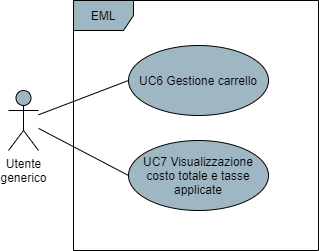
\includegraphics[scale=0.6]{res/UseCase/Immagini/CarrelloGenerale}
\caption{Diagramma UML per modulo del carrello}
\end{figure}

\subsubsection{UCX - Gestione Carrello}
\begin{itemize}
\item \textbf{Attori primari}:
\item \textbf{Attori secondari}:
\item \textbf{Descrizione}:
\item \textbf{Scenario Principale}:
\item \textbf{Estensioni}:
\item \textbf{Specializzazioni}:
\item \textbf{Precondizione}:
\item \textbf{Postcondizione}:
\end{itemize}

\begin{figure}[H]
\centering
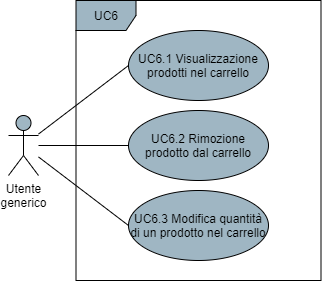
\includegraphics[scale=0.6]{res/UseCase/Immagini/GestioneCarrello}
\caption{Diagramma UML per UCX - Gestione carrello}
\end{figure}

\subsubsection{UCX.1 - Visualizzazione prodotti nel carrello}
\begin{itemize}
\item \textbf{Attori primari}:
\item \textbf{Attori secondari}:
\item \textbf{Descrizione}:
\item \textbf{Scenario Principale}:
\item \textbf{Estensioni}:
\item \textbf{Specializzazioni}:
\item \textbf{Precondizione}:
\item \textbf{Postcondizione}:
\end{itemize}

\subsubsection{UCX.2 - Rimozione prodotto nel carrello}
\begin{itemize}
\item \textbf{Attori primari}:
\item \textbf{Attori secondari}:
\item \textbf{Descrizione}:
\item \textbf{Scenario Principale}:
\item \textbf{Estensioni}:
\item \textbf{Specializzazioni}:
\item \textbf{Precondizione}:
\item \textbf{Postcondizione}:
\end{itemize}

\subsubsection{UCX.3 - Modifica quantità di un prodotto nel carrello}
\begin{itemize}
\item \textbf{Attori primari}:
\item \textbf{Attori secondari}:
\item \textbf{Descrizione}:
\item \textbf{Scenario Principale}:
\item \textbf{Estensioni}:
\item \textbf{Specializzazioni}:
\item \textbf{Precondizione}:
\item \textbf{Postcondizione}:
\end{itemize}

\subsubsection{UCX.4 - Visualizzazione costo totale del carrello}
\begin{itemize}
\item \textbf{Attori primari}:
\item \textbf{Attori secondari}:
\item \textbf{Descrizione}:
\item \textbf{Scenario Principale}:
\item \textbf{Estensioni}:
\item \textbf{Specializzazioni}:
\item \textbf{Precondizione}:
\item \textbf{Postcondizione}:
\end{itemize}

\subsubsection{UCX.5 - Visualizzazione tasse applicate nel carrello}
\begin{itemize}
\item \textbf{Attori primari}:
\item \textbf{Attori secondari}:
\item \textbf{Descrizione}:
\item \textbf{Scenario Principale}:
\item \textbf{Estensioni}:
\item \textbf{Specializzazioni}:
\item \textbf{Precondizione}:
\item \textbf{Postcondizione}:
\end{itemize}




